\subsection{Dark matter}
\label{sec:DM}
We have many unanswered mysteries in physics today, but probably the greatest one is the nature of dark matter (DM) \cite{monoZexclusion}. In the previous section's SUSY processes, we have seen that a "consequence" of SUSY may give us some viable DM candidates, namely the LSP neutralino. In this section, we will look at DM particles produced in a more simplified model; that is, a non-supersymmetry model. In this model, we assume that we have a DM mediator in addition to the DM particles in the final state. This mediator can be, among others, a scalar or a vector. This process's signature consists of detecting a well known SM particle recoiling against missing energy-momentum carried away by DM particles. 





\begin{comment}
\textbf{To do:}
\begin{itemize}
    \item Les om mørk materie. Du har jo strengt tatt ikke litt peiling engang..
    \item 
\end{itemize}


\begin{figure}[H]
    \centering
    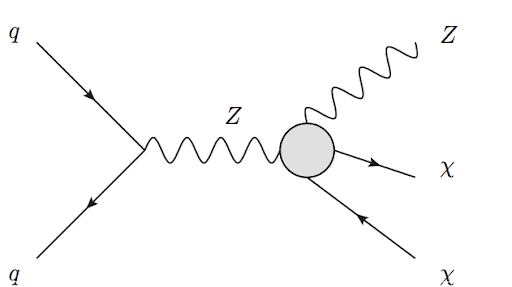
\includegraphics[width = 0.5\textwidth]{Figures/FeynmanDiagrams/monoZFeynman1.png}
    \caption{Caption}
    \label{fig:monoZFeynman1}
\end{figure}
\end{comment}






